\documentclass{article}
\usepackage{graphicx}
\usepackage{multirow}
\usepackage{float}
\usepackage{pbox}
\usepackage{siunitx}
\usepackage{geometry}
\usepackage{adjustbox}
\usepackage[numbers]{natbib}
\title{Supplementary Materials}

\author{Justin K. Miller, Tristram J. Alexander}


\begin{document}



\maketitle

\section{Correlation between metrics}
To better understand how each automated metric compares, we calculated the Pearson rank correlation for each pair of metrics based on their scores within each cluster, as presented in the heatmap (see  Fig. S\ref{fig:Metric}). Notably, silhouette scores showed a correlation exclusively with the mean standard deviation. This correlation is logical given that both metrics aim to measure similar aspects. However, the silhouette scores' low correlation with other metrics is unexpected. In contrast, Keywords and Distance metrics exhibited a significant correlation, aligning with their common goal of assessing cluster distinctiveness. Despite their different approaches, this correlation validates their effectiveness as tools for measuring the uniqueness of clusters. 






\begin{figure}[htbp]
 \begin{flushleft}
  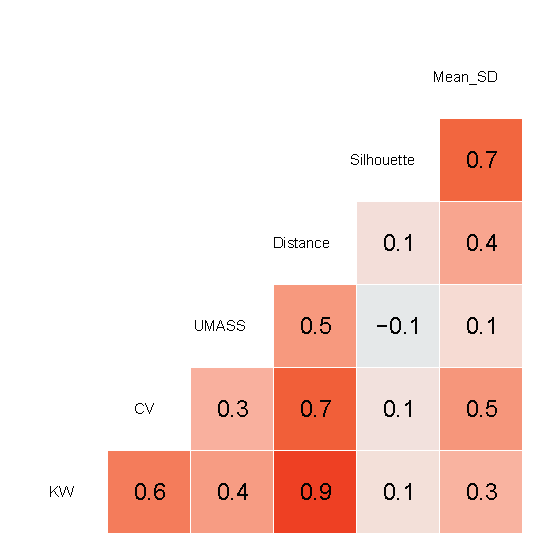
\includegraphics[width=0.8\linewidth]{Figures/Metric_Correlation_new.eps}
  \caption{This figure shows the Pearson rank correlation between each of the automated metric scores for each of the 40 clusters.(KW is short for number of Keywords in a cluster)}
  \label{fig:Metric}
  \end{flushleft}
\end{figure}



\section{UMAP Visualisation}
To effectively visualize the relationships between different clusters in our 384-dimensional large language model dataset, we employed Uniform Manifold Approximation and Projection (UMAP) for dimensionality reduction \cite{mcinnes2018umap}, see Fig.S~\ref{fig:UMAP}. The choice of UMAP is particularly pertinent due to its exceptional ability to retain the topology of the data, a feature crucial for our objective of illustrating the spatial relationships between various bios. Unlike Principal Component Analysis (PCA), which primarily captures linear relationships and variance, UMAP excels in preserving both the local and global structures within the data. This is especially important given that our dataset exhibits orthogonal dimensions, as evidenced by the correlation plot in Fig.S \ref{fig:correlation_matrix}. Although PCA might typically be effective in scenarios with orthogonal dimensions, its linear approach could potentially overlook the more complex, non-linear relationships present in our data. Therefore, UMAP's capacity to handle non-linear structures makes it a more suitable choice for our analysis, ensuring a more accurate and insightful two-dimensional representation of the clusters. The results of this can be seen in Fig.S \ref{fig:UMAP}.




\begin{figure}[H]
\centering
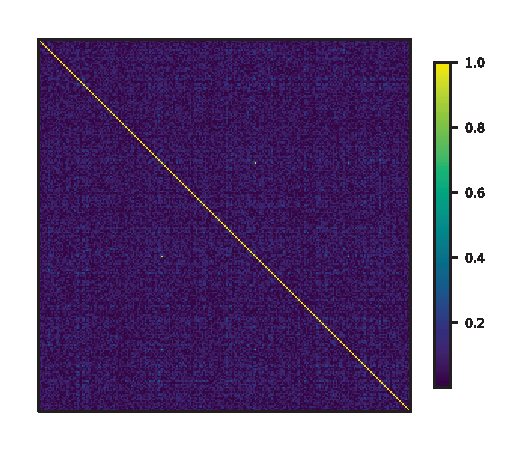
\includegraphics[width=\linewidth]{Figures/correlation_matrix.eps}
\caption{Pearson Correlation between all 384 vectors in the LLM}
\label{fig:correlation_matrix}
\end{figure}


\begin{figure}[htbp]
 \begin{flushleft}
  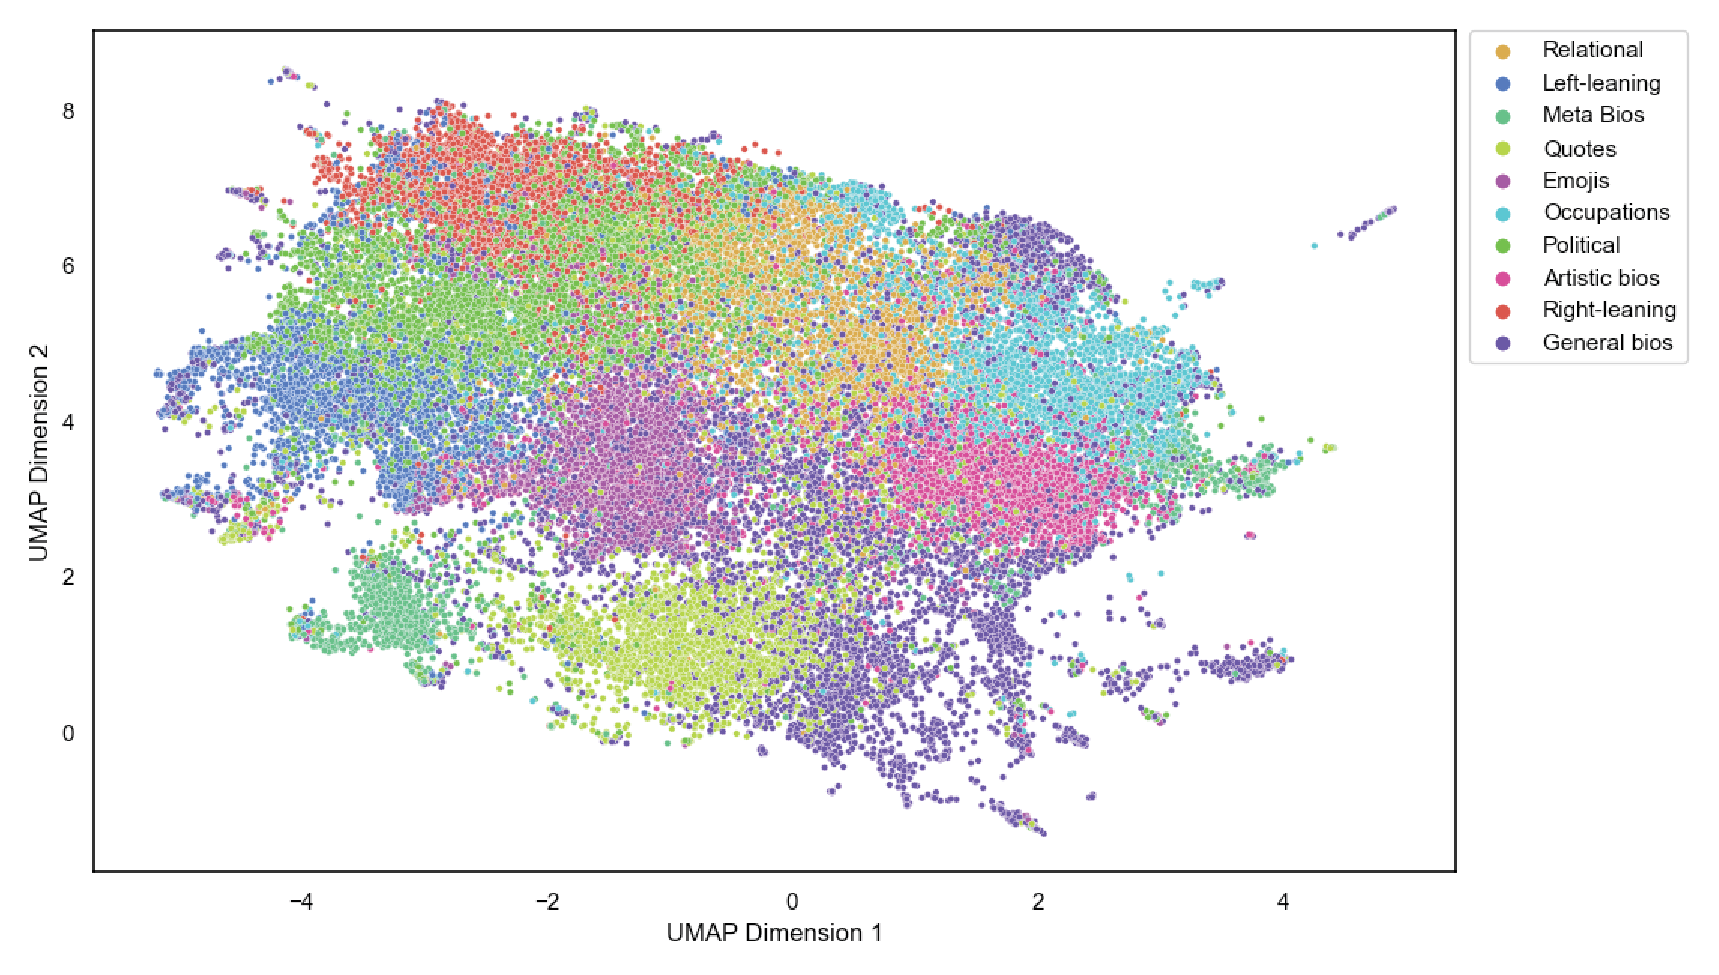
\includegraphics[width=0.8\linewidth]{Figures/Clustering}
  \caption{This figure shows all 38k Twitter bios projected onto a 2d plane using UMAP to show each points relation to each other, and which clusters are more similar to each other}
  \label{fig:UMAP}
  \end{flushleft}
\end{figure}





\section{Stability}

The three models used in the main paper each incorporate a stochastic component, which means that they can yield entirely different clusters with each run.To assess the stability of our methods, we executed them using various random seeds. For each seed, we calculated the pairwise Adjusted Mutual Information (AMI) between each seed. Our findings revealed that the LDA model had an average AMI of 0.25, with a standard deviation of 0.02. In contrast, the Doc2vec Model exhibited an average AMI of 0.91 and a standard deviation of 0.07, while the LLM showed an average AMI of 0.79 with a standard deviation of 0.09. The distribution of the AMI between each seed can be seen in  In figures S\ref{fig:LDA_Stability}, S\ref{fig:Doc2vec_Stability}, and S\ref{fig:LLM_Stability}. LDA appears to be a normal distribution. This seems to indicate that in all 50 seeds, none of them had similarly labelled clusters. This calls into question the reliability of LDA and its implementation in short text. The GMM approaches seem to be quite a lot higher, both of them seem to have around 3 peaks (a small fourth in Doc2vec), potentially indicating that there are three local maxima that the algorithm finds. All three of them seem to have a high AMI indicating they are fairly similar. However, this needs to be further explored to test what tangible differences, if any, there are between these three maxima.








\begin{figure}[H]
\centering
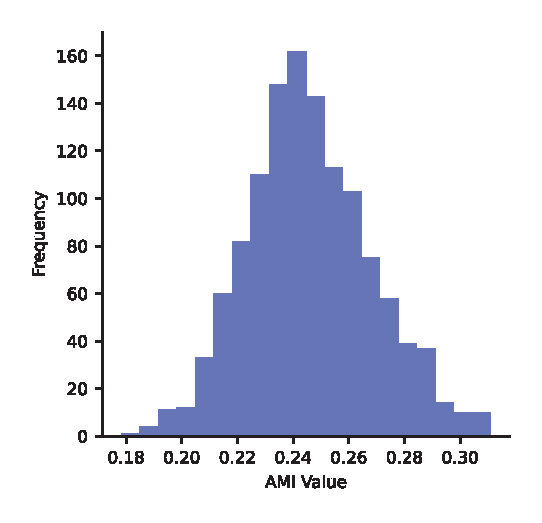
\includegraphics[width=0.9\linewidth]{Figures/LDA_Stability.eps}
\caption{Distribution of pairwise AMI between 50 different seeds of LDA implementation}
\label{fig:LDA_Stability}
\end{figure}



\begin{figure}[H]
\centering
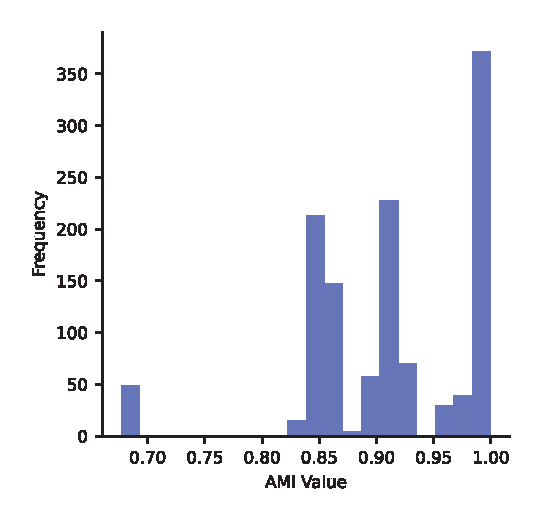
\includegraphics[width=0.9\linewidth]{Figures/Doc2vec_Stability.eps}
\caption{Distribution of pairwise AMI between 50 different seeds of GMM implementation using vectors created by Do2vec}
\label{fig:Doc2vec_Stability}
\end{figure}



\begin{figure}[H]
\centering
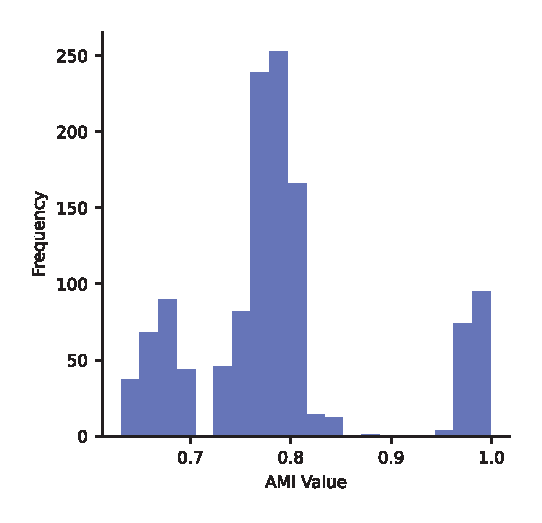
\includegraphics[width=0.9\linewidth]{Figures/LLM_Stability.eps}
\caption{Distribution of pairwise AMI between 50 different seeds of GMM implementation using vectors created by a LLM}
\label{fig:LLM_Stability}
\end{figure}



\section{Other Models of ChatGPT}
The use of ChatGPT allows us to explore effects which would be resource-intensive when using human reviewers.  
To evaluate ChatGPT's performance with an increased number of bios, we conducted tests using 20, 100, and 500 bios as input, focusing on clusters that represented a range in diversity. This was done to assess the model's scalability while managing costs, so we limited our tests to two clusters per method.  The procedure was consistent with our earlier experiments using the ChatGPT API, with no alterations besides the number of bios, and using GPT-4 Turbo as it can take more bios \cite{openai_2023}. After processing the bios through ChatGPT-4 Turbo, we applied the same analysis method from Section 3.8, of the method section in the main paper, to determine the frequency of the most commonly used word in the generated names. Rather than naming all clusters, we choose a small subset of clusters from across the models.  We can see in Fig.S~\ref{fig:gpt_Name} that increasing the number of bios does not appear to lead to a systematic change in the accuracy of the names produced by ChatGPT. 

\begin{figure}[htbp]
 \begin{flushleft}
  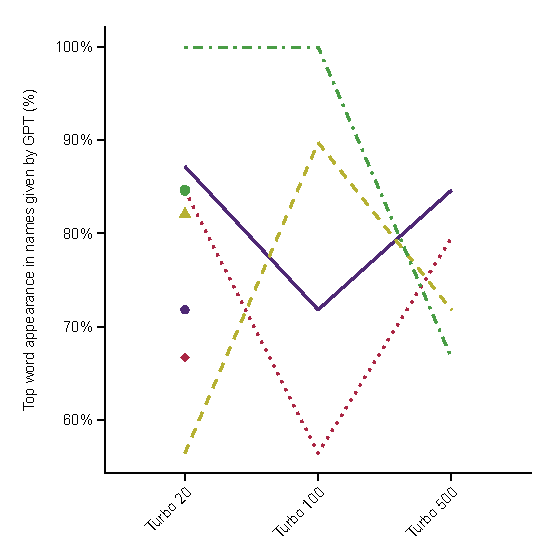
\includegraphics[width=0.9\linewidth]{Figures/GPT_model_naming.eps}
  \caption{This figure shows the different levels of relability between gpt-4 being given 20 bios (symbols), and gpt-turbo being given 20, 100, and 500 bios, and being asked to name it.}
  \label{fig:gpt_Name}
  \end{flushleft}
\end{figure}






\section{Process Pipeline}







\begin{figure}[H]
\centering
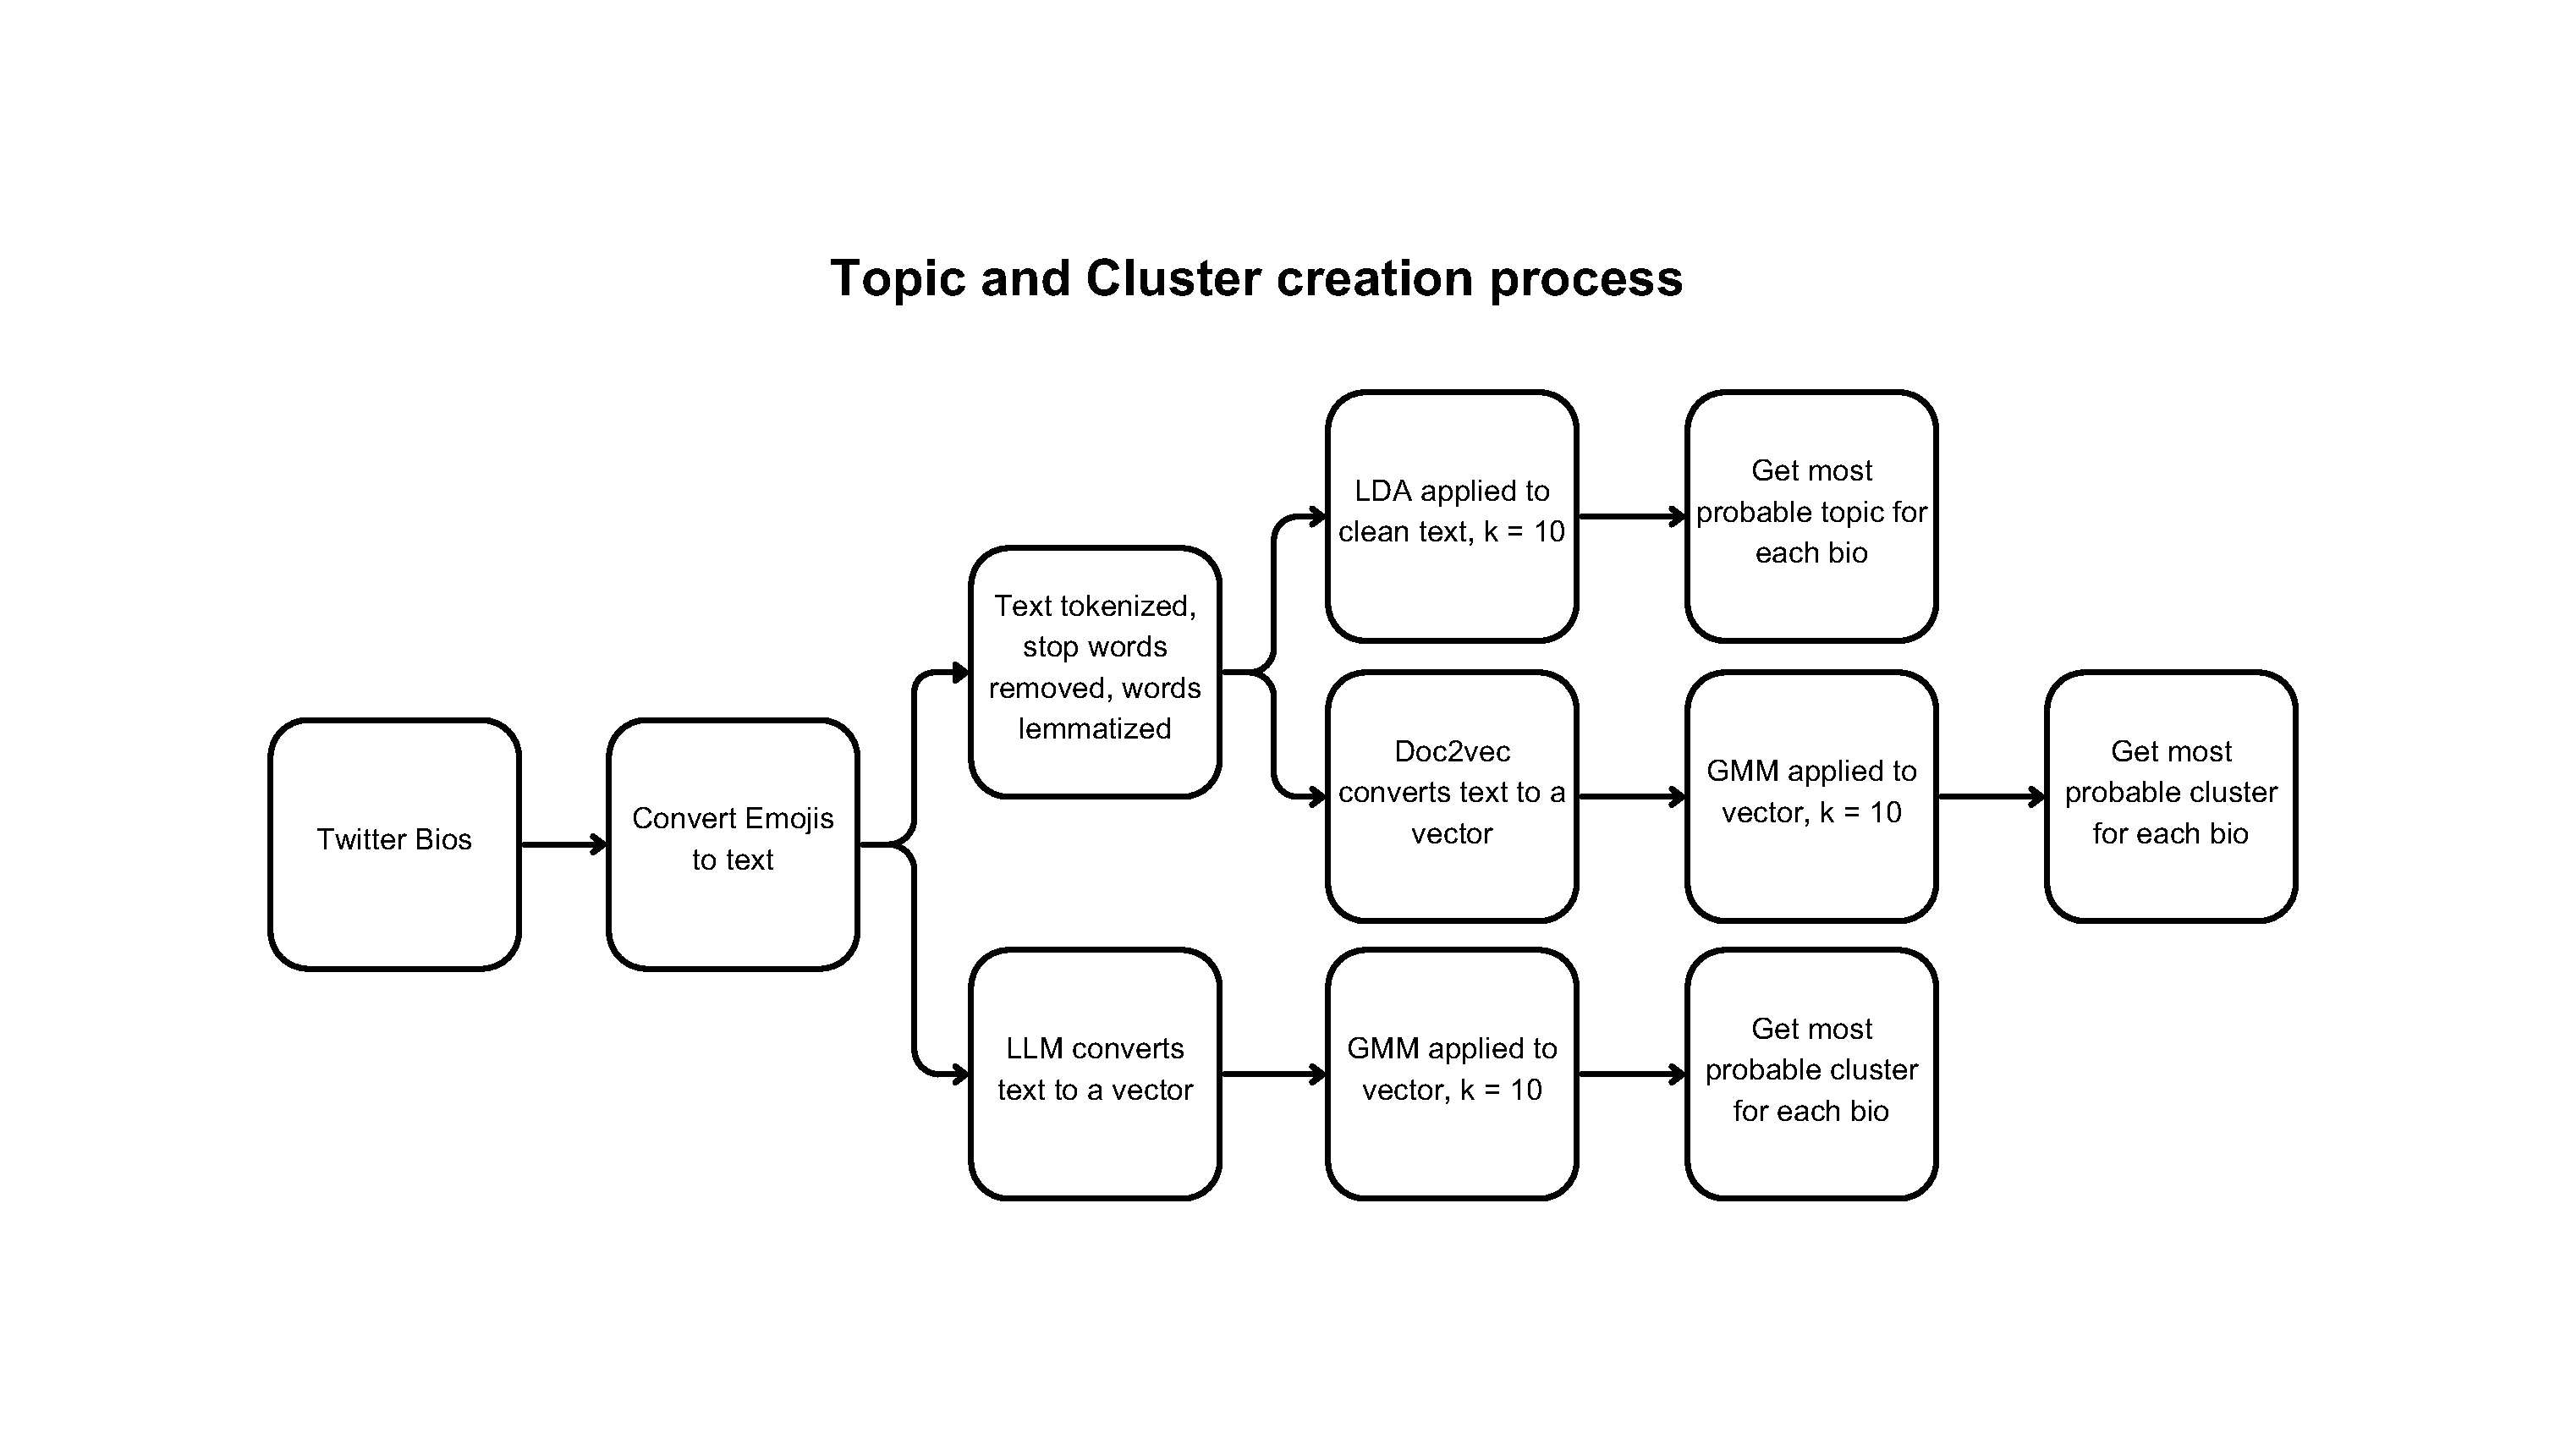
\includegraphics[width=0.9\linewidth]{Figures/Twitter_Bios.eps}
\caption{Diagram showing the process to building each model}
\label{fig:Twitter_Bios}
\end{figure}



\begin{figure}[H]
\centering
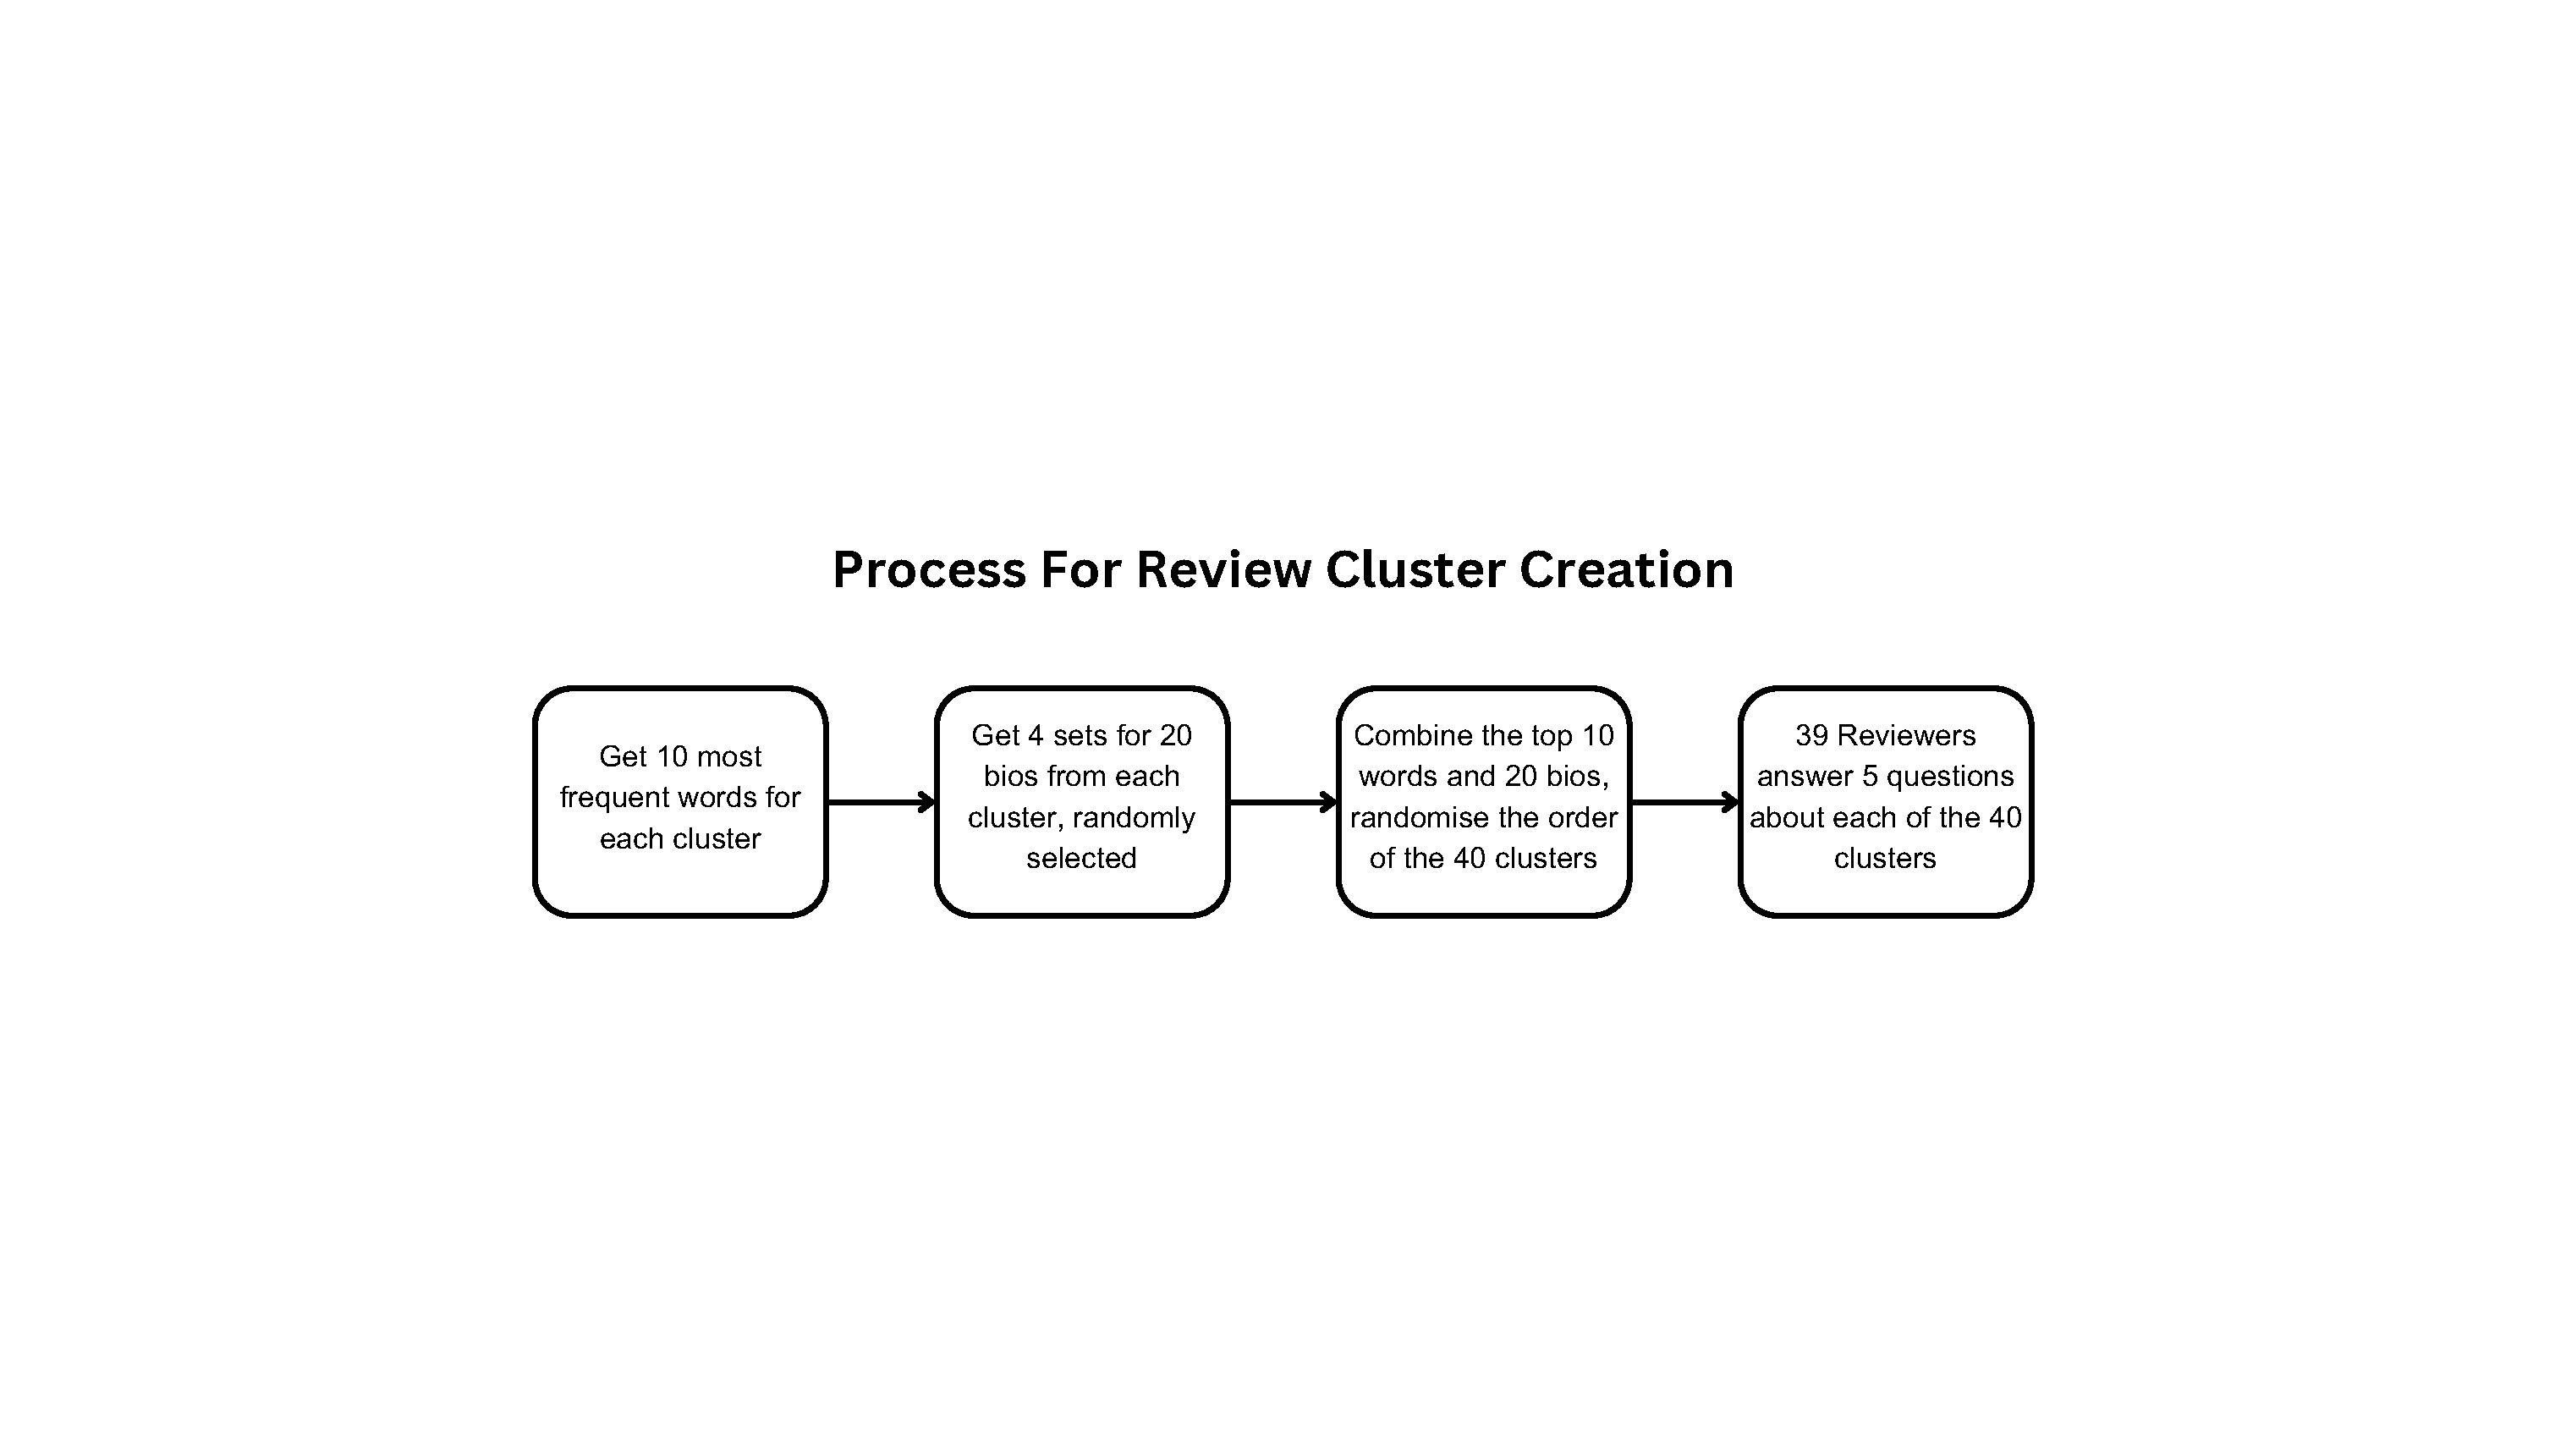
\includegraphics[width=0.9\linewidth]{Figures/Get_10_most_frequent_words_for_each_cluster.eps}
\caption{Diagram showing the process by which the cluster samples were created to show to our reviewers}
\label{fig:Review_Process}
\end{figure}




The pipeline for how each cluster was created to show to our reviewers is in Fig.S \ref{fig:Review_Process}
The reviewers are shown each cluster in a random order and are not told which model a cluster came from. For each
of the 40 clusters, reviewers must read the top 10 words and the 20 sample bios
and then answer the following questions:
\begin{itemize}
    \item ``Create a name using less than 10 words to summarize the top 10 words/emojis and the sample bios of the Sample Cluster. If you believe it is not possible to do this with a cluster, write `None'.'' This gives a summary of whether the cluster is human-interpretable and a description of the types of bios in the cluster.
    
    \item ``When you named a Sample Cluster, were you confident that the name summarized the whole cluster?'' Reviewers can answer this question by selecting one of the following: Not at all Confident/Not Confident/Neutral/Confident/Very Confident. This question helps understand how easy it was to understand each cluster.
    
    For the following questions, reviewers can respond with: Strongly disagree/ Disagree / Neutral / Agree / Strongly Agree
    
    \item ```The situation when the top words/emojis of a cluster fit together in a natural or reasonable way' Do you agree that the above statement describes the top words/emojis of this Sample Cluster?'' This question tests whether the top 10 words/emojis of a cluster are coherent.
    
    \item ```The situation when the Sample bios of a cluster fit together in a natural or reasonable way' Do you agree that the above statement describes the sample bios of this Sample Cluster?'' This question tests whether the sample bios of each cluster are coherent.
    
    \item ```The Top Words/Emojis provide an accurate summary of the sample bios' Do you agree that the above statement describes this Sample Cluster?'' This tests if the top words/emojis and sample bios are coherent with each other.
\end{itemize}

The data given by the reviewers was then ingested and cleaned. The responses to the questions above were converted to a 1-5 scale, where a 5 represents ``Strongly Agree" or ``Very Confident" and a 1 represents ``Strongly Disagree" or ``Not at All Confident". For the confidence in naming question, some reviewers were unable to name the cluster but gave it a score of 4 or 5. In these cases, the data was changed so that every cluster that had ``None" for its name was given a score of 1 for the question on confidence in naming.

This study had ethics approval from the University of Sydney. Reviewers were sourced from Prolific and responses were collected through Redcap. We collected 40 reviewers, however, had to exclude one due to them misunderstanding the prompt and copying and pasting bios as the names for each cluster, as well as a non-serious attempt at the other questions. An example of how a reviewer saw each cluster can be seen in figures S\ref{fig:Screenshot 1} and S\ref{fig:Screenshot 2}


\begin{figure}
\includegraphics[width=0.9\linewidth]{Figures/Cluster1_Bios1.eps}
\caption{Screenshot from Redcap of the reviewer being shown the contents of each cluster}
\label{fig:Screenshot 1}
\end{figure}


\begin{figure}
\includegraphics[width=0.9\linewidth]{Figures/Cluster_1_Bios_question.eps}
\caption{Screenshot from Redcap of the reviewer being shown the questions and where they input their answers. Same cluster as the previous figure}
\label{fig:Screenshot 2}
\end{figure}



\section{Inter-Coder Reliability}
Inter-coder reliability measures the agreement between reviewers which is important given the subjective nature of their task. If there is low inter-coder agreement, this calls into question the interpretability of the clusters regardless of any other analysis. Since the data is ordinal and reviewers rate every single cluster, the appropriate method to use is the Intraclass Correlation Coefficient (ICC) \cite{gisev2013interrater, mcgraw1996forming}. The ICC is a number between 0 and 1, with a higher number indicating greater agreement between reviewers. To provide context for the ICC scores, Koo et al. provided a guideline \cite{koo2016guideline}: a score less than 0.5 is poor, a score between 0.5-0.75 is moderate, a score between 0.75-0.9 is good, and a score above 0.9 is excellent.

ICC estimates and their 95\% confident intervals were calculated using R version 4.2.2 \cite{rsoftware2022} and the 
statistical package Psych version 2.2.9 \cite{psych2022} based on an average rating, two-way random effects, absolute agreement, multiple raters/measurements. Table S\ref{table:1} shows the results of the results for each of the questions reviewers were asked.

\newgeometry{left=0.5cm, right=0.5cm}
\begin{table*}
\small
  \centering
  \begin{tabular}{|l|l|l|l|l|l|l|l|}
    \hline
    \multirow{2}{*}{Metric} &
      \multicolumn{1}{c|}{Intraclass Correlation} &
      \multicolumn{2}{c|}{95\% Confidence Interval} &
      \multicolumn{4}{c|}{F Test with True Value 0} \\
      \cline{3-8}
      & & Lower Bound & Upper Bound & Value & df1 & df2 & Sig \\
    \hline
    Confidence in Naming & .900 & .0849 & .94 & 13.5 & 39 & 1482 & \num{9.3e-73} \\
    \hline
    Coherence of Top Words & .922 & .883 & .953 & 14.7 & 39 & 1482 & \num{1.3e-79} \\
    \hline
    Coherence of Sample Bios & .911 & .866 & .946 & 13.7 & 39 & 1482 & \num{1.5e-73} \\
    \hline
    Coherence between Top Words and Sample Bios & .926 & .889 & .955 & 15.7 & 39 & 1482 & \num{7.1e-85} \\
    \hline
  \end{tabular}
  \caption{ICC Calculation in R Using Two-way random, average measure (ICC(2,k))}
  \label{table:1}
\end{table*}
\restoregeometry
From this it can be seen that the ICC is considered excellent across all four questions, indicating that the reviewers were in relative agreement on their ratings of each cluster.  A limitation of this method is that it assumes that the data is continous, but the reviewer responses are ordinal.




\section{Automated Methods}



\subsection{Automated Metric Results}
The results for every cluster's automated metrics can be found in table S\ref{table:Automated_table}
Using the automated measures to judge and compare each of the 4 models, every automated metric except for  $C_{UMASS}$ agrees with the ranking given by human reviewers: LLM, LDA, Doc2vec, and Random. However, when looking at the ranking of the individual clusters there is a much greater difference. Overall it seems that all the automated methods fail when looking at individual clusters, but in a small sample of 4 models can rank them effectively.

\subsubsection{Coherence}
Both coherence methods found that LDA 1 was the most coherent, this was in contrast to the reviewers who were not able to name the cluster and gave on average quite low scores across the 4 questions. Doc2vec had comparatively good $C_{UMASS}$ scores. In terms of $C_V$, it scored generally lower, with its highest score being for Doc2vec 4 which was one of the few that reviewers were able to consistently name. The LLM clusters that were political in nature (0,2, and 9) scored quite well on the coherence metrics, however, other clusters that were rated quite high by reviewers were given low scores. On the whole, it does not appear that either metric of coherence matches up with human interpretability. 


\subsubsection{Cluster Distance}
The results from all models show low silhouette scores, with the majority of the scores close to zero. The reason for this is because of the high standard deviation in each dimension from the embeddings generated for the LLM and used to generate the silhouette score for all four models. Fig.S \ref{fig:Silhouette} shows that with synthetic data, the clusters generated by a GMM are able to match the silhouette score of the true clusters. As standard deviation increases it can be seen that the silhouette score decreases even amongst the true label. So the low silhouette scores are not a reflection of bad clustering but rather high standard deviation in the data. 

\begin{figure*}
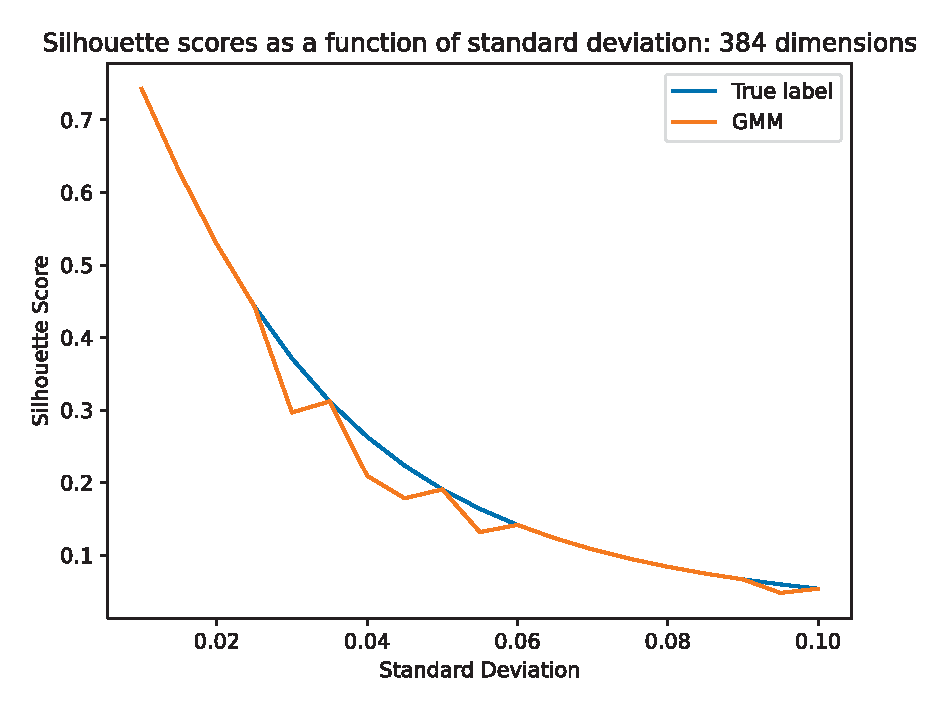
\includegraphics[width=0.9\linewidth]{Figures/Silhouette_SD.eps}
\caption{Silhouette Score as Standard deviation increases on Synthetic data}
\label{fig:Silhouette}
\end{figure*}



\subsubsection{Keyword Analysis}
Keyword analysis showed vast differences between the three models in terms of lexical content. On average, the transformer model created the clusters with the most keywords and highest average keyness scores. In more practical terms, this implies that the transformer model created the clusters that were most distinct from the original corpus of bios in terms of word frequency. In contrast, Doc2Vec was by far the worst-performing model, including several clusters with no keywords. This implies that the distribution of words in said clusters is near identical to the original corpus. Therefore, to make clusters that are lexically distinct from one another, the Transformer model performs the best.






\newgeometry{left=0.5cm, right=0.5cm}
\begin{table}[!ht]
\small
    \centering
    \begin{tabular}{|p{2cm}|p{2cm}|p{6cm}|p{1.2cm}|p{1cm}|p{1cm}|p{1.1cm}|p{1.3cm}|p{1cm}|}
    \hline
        Cluster id & Name & GPT Name & Keywords & CV & UMASS  & Distance & Silhouette & Mean SD \\ \hline
        Doc2vec 0 & U1 & Political Views and Personal Attitudes & 0 & 0.26 & -3.5 & 0.012 & -0.033 & 0.048 \\ \hline
        Doc2vec 1 & U2 & Minimal Information MAGA Supporters & 32 & 0.2 & -2.1 & 0.053 & 0.004 & 0.047 \\ \hline
        Doc2vec 2 & U3 & Diverse Personal Interests and Beliefs & 5 & 0.29 & -4 & 0.012 & -0.035 & 0.047 \\ \hline
        Doc2vec 3 & U4 & Varied Interests and Political Opinions & 62 & 0.33 & -2.6 & 0.022 & -0.024 & 0.047 \\ \hline
        Doc2vec 4 & Political\_1 & Mixed Political Sentiments and Personal Interests & 8 & 0.45 & -3.3 & 0.002 & -0.021 & 0.046 \\ \hline
        Doc2vec 5 & U5 & Mixed Political Views & 0 & 0.26 & -3.5 & 0.005 & -0.026 & 0.047 \\ \hline
        Doc2vec 6 & Political\_2 & Mixed Political Sentiments & 0 & 0.34 & -3.6 & 0.003 & -0.023 & 0.046 \\ \hline
        Doc2vec 7 & U6 & Diverse Political Interests & 0 & 0.27 & -8.3 & 0.004 & -0.010 & 0.046 \\ \hline
        Doc2vec 8 & U7 & Personal Interests and Political Affiliations & 0 & 0.44 & -8.8 & 0.004 & 0.011 & 0.045 \\ \hline
        Doc2vec 9 & U8 & Political Perspectives and Personal Interests & 0 & 0.42 & -4.4 & 0.002 & -0.022 & 0.046 \\ \hline
        LDA 0 & Left leaning\_1 & Activists and Biden Supporters & 38 & 0.35 & -2.7 & 0.086 & -0.015 & 0.045 \\ \hline
        LDA 1 & U9 & Personal Perspectives and Interests & 42 & 0.69 & -4 & 0.082 & -0.050 & 0.047 \\ \hline
        LDA 2 & U10 & Diverse Interests and Professions & 39 & 0.25 & -2.9 & 0.037 & -0.060 & 0.048 \\ \hline
        LDA 3 & Right Leaning & Patriotic Trump Supporters & 39 & 0.62 & -2.7 & 0.115 & 0.107 & 0.042 \\ \hline
        LDA 4 & Relationships & Family and Occupation Focus & 58 & 0.36 & -2.8 & 0.076 & -0.005 & 0.045 \\ \hline
        LDA 5 & U11 & Opinion Expressers & 54 & 0.42 & -3.3 & 0.049 & -0.047 & 0.048 \\ \hline
        LDA 6 & U12 & Veterans and Varied Interests & 32 & 0.31 & -2.3 & 0.043 & -0.059 & 0.047 \\ \hline
        LDA 7 & U13 & Varied Interests and Political Engagement & 51 & 0.31 & -2.7 & 0.052 & -0.039 & 0.046 \\ \hline
        LDA 8 & U14 & American Sociopolitical Views and Beliefs & 55 & 0.35 & -2.8 & 0.061 & -0.056 & 0.046 \\ \hline
        LDA 9 & Left leaning\_2 & Life, Politics, and Personal Interests & 60 & 0.35 & -2.6 & 0.037 & -0.062 & 0.047 \\ \hline
        LLM 0 & Left Leaning & Democratic Supporters and Resisters & 131 & 0.54 & -2.6 & 0.222 & 0.028 & 0.041 \\ \hline
        LLM 1 & Artistic Bios & Creative Professionals and Enthusiasts & 230 & 0.4 & -3.2 & 0.246 & 0.033 & 0.044 \\ \hline
        LLM 2 & Political & Political Affiliation and National Pride & 155 & 0.56 & -2.8 & 0.246 & -0.029 & 0.043 \\ \hline
        LLM 3 & Occupations & Professionals and Students with Various Interests & 264 & 0.29 & -4.1 & 0.183 & 0.008 & 0.045 \\ \hline
        LLM 4 & Relational & Family-oriented Patriotic Individuals & 129 & 0.38 & -2.9 & 0.304 & 0.074 & 0.042 \\ \hline
        LLM 5 & General & Eclectic Personal Expressions & 191 & 0.37 & -7.7 & 0.222 & -0.070 & 0.048 \\ \hline
        LLM 6 & Twitter & Twitter-focused Political Commentators & 133 & 0.45 & -8.1 & 0.162 & 0.035 & 0.043 \\ \hline
        LLM 7 & Quotes & Life Philosophies and Personal Beliefs & 270 & 0.43 & -7.7 & 0.334 & -0.019 & 0.046 \\ \hline
        LLM 8 & Right Leaning & Patriotic Trump Supporters & 224 & 0.7 & -1.9 & 0.291 & 0.160 & 0.038 \\ \hline
        LLM 9 & Emojis & Polarized Political Users & 216 & 0.48 & -2.6 & 0.162 & 0.099 & 0.041 \\ \hline
        Random 0 & U15 & Political Interests and Personal Identities & 1 & 0.05 & -5.1 & 0.001 & -0.002 & 0.046 \\ \hline
        Random 1 & U16 & Diverse Political and Personal Interests & 1 & 0.08 & -4.1 & 0.001 & -0.003 & 0.046 \\ \hline
        Random 2 & U17 & Polarized Political Views & 0 & 0.15 & -5 & 0.001 & -0.002 & 0.046 \\ \hline
        Random 3 & U18 & Political Standpoints and Diverse Interests & 0 & 0.09 & -4.6 & 0.001 & -0.003 & 0.046 \\ \hline
        Random 4 & U19 & Mixed MAGA Supporters and Resistors & 0 & 0.21 & -4.2 & 0.001 & -0.001 & 0.046 \\ \hline
        Random 5 & U20 & Mixed Political Views and Personal Interests & 2 & 0.13 & -4.3 & 0.001 & -0.005 & 0.047 \\ \hline
        Random 6 & U21 & Diverse Personal Interests and Politics & 1 & 0.18 & -4.2 & 0.001 & -0.002 & 0.046 \\ \hline
        Random 7 & U22 & American Politics and Personal Interests & 0 & 0.25 & -5 & 0.001 & -0.005 & 0.047 \\ \hline
        Random 8 & U23 & Mixed Political Sentiments & 0 & 0.24 & -4.2 & 0.001 & -0.003 & 0.046 \\ \hline
        Random 9 & U24 & Political Views and Personal Interests & 0 & 0.14 & -4.7 & 0.001 & -0.001 & 0.046 \\ \hline
    \end{tabular}
    \caption{Table showing every clusters score for each automated metric, including how it was named by one example use of Chatgpt}
    \label{table:Automated_table}
\end{table}
\restoregeometry



\subsection{Naming Of Clusters}

The top words that were given to each reviewer are shown in Table S\ref{table:top_words}. The LLM model appears to have a greater range of different types of bios, where the Doc2vec model only has clusters that are related to politics, and the LDA model only has 2 that are non-political, the LLM model has 5 clusters that are non-political. It also has no clusters that were not able to be named.


It can be seen that in figures S\ref{fig:LDA_Names}, S\ref{fig:Doc2vec_Names},  S\ref{fig:Random_Names}
reviewers were unable to name the LDA, Doc2vec, and Random clusters at a much lower rate than the LLM model, as evidenced by the increased use of the word "None" across those three clusters. In the clusters that were not able to be named (designated by a U), ChatGPT seems to do what the reviewers tend to do and name it based on being political. It is of note that while ChatGPT was instructed to write "None" if a cluster did not appear to have any meaning, it never did. This demonstrates a potential flaw in using ChatGPT to name clusters.

\begin{figure*}
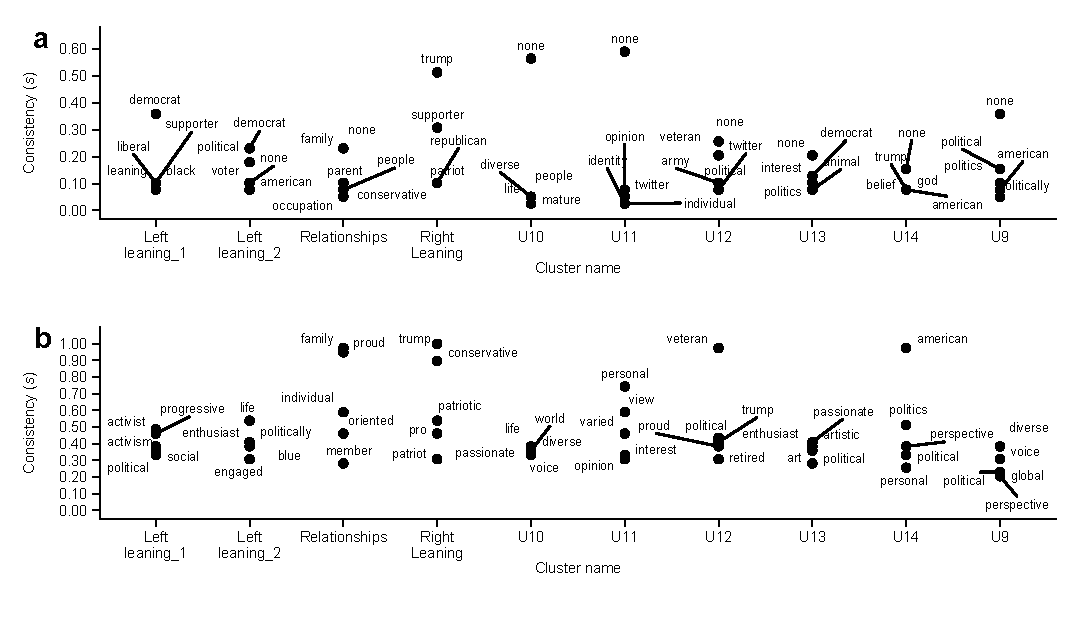
\includegraphics[width=0.9\linewidth]{Figures/Reviewer_Names_Graph_LDA.eps}
\caption{The top five words by fraction of appearance used by (a) reviewers and (b) ChatGPT to name the clusters created by the LDA. Along the x-axis are the names given to each cluster by the authors of this paper.}
\label{fig:LDA_Names}
\end{figure*}


\begin{figure*}
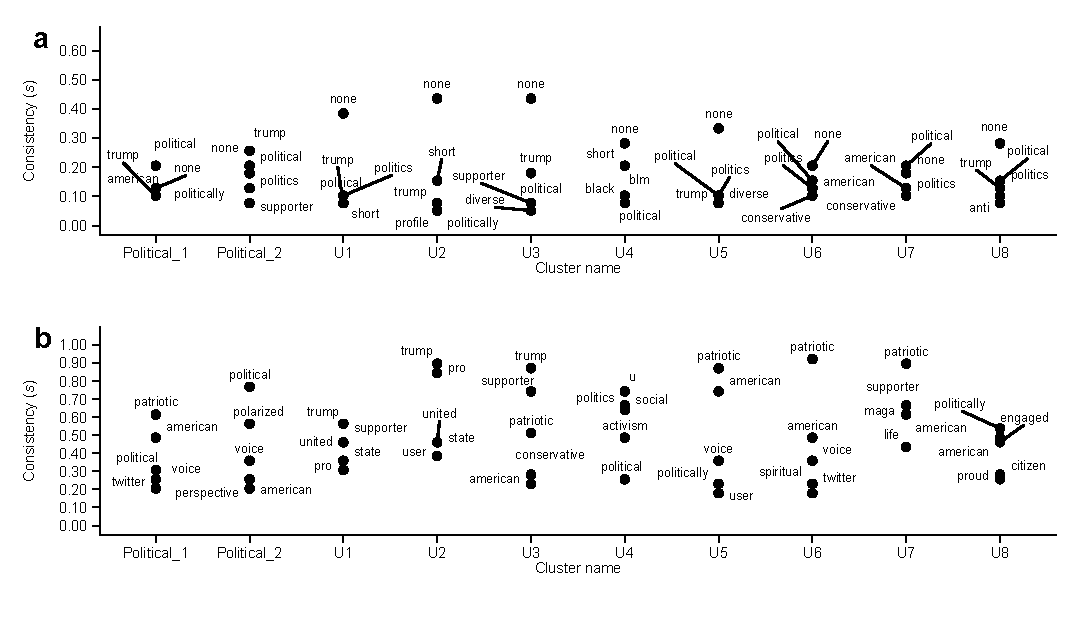
\includegraphics[width=0.9\linewidth]{Figures/Reviewer_Names_Graph_Doc2vec.eps}
\caption{The top five words by fraction of appearance used by (a) reviewers and (b) ChatGPT to name the clusters created by Doc2vec. Along the x-axis are the names given to each cluster by the authors of this paper.}
\label{fig:Doc2vec_Names}
\end{figure*}
  We see that the words used to describe the clusters are largely consistent between ChatGPT and the reviewers, however there are cluster-dependent distinctions revealing human and machine limitations as discussed in the text.

\begin{figure*}
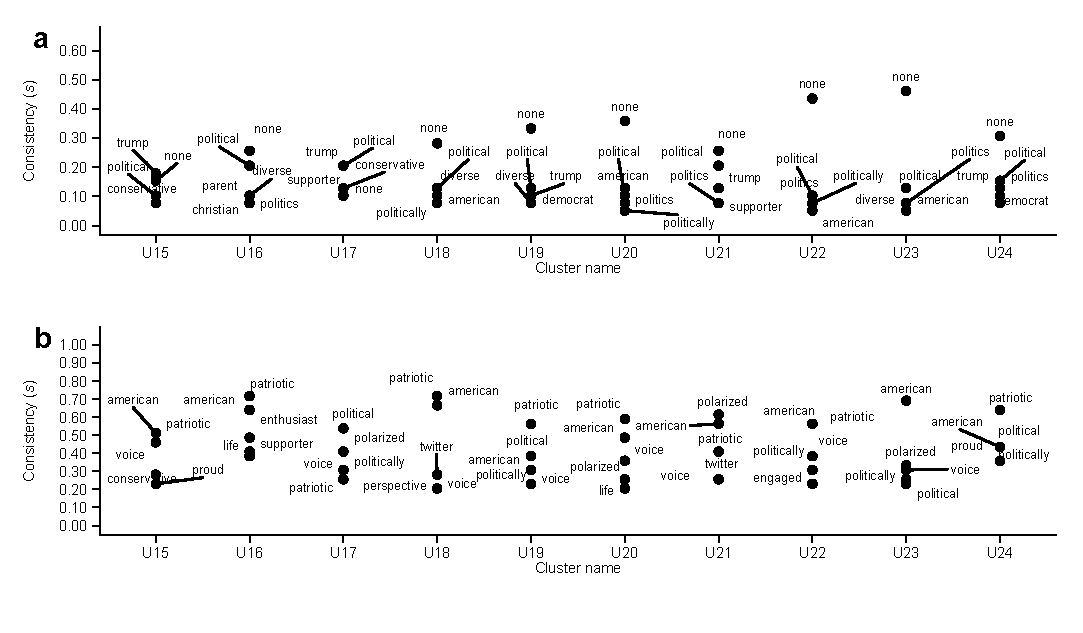
\includegraphics[width=0.9\linewidth]{Figures/Reviewer_Names_Graph_Random.eps}
\caption{The top five words by fraction of appearance used by (a) reviewers and (b) ChatGPT to name the clusters created by the Random Model. Along the x-axis are the names given to each cluster by the authors of this paper.}
\label{fig:Random_Names}
\end{figure*}



From examining each model at a cluster level, the LLM model appears to create a wider range of different clusters, that are more robustly interpretable by the reviewers.


\newgeometry{left=0.5cm, right=0.5cm}
\begin{table}[h!]
\centering
\begin{tabular}{|l|l|p{13cm}|} 
 \hline
 Cluster ID & Cluster Name & Top 10 Frequent Words \\ [0.5ex] 
 \hline
 LDA 0 & Left leaning 1 & Resist, Blm, Http, Blacklivesmatter, Matter, Life, Black, Bidenharris2020, Fbr, Theresistance \\ \hline 
 LDA 1 & Undecided & New, Side, Party, Local, National, flag-mexico, Analyst, Troll, Old, General \\ \hline
 LDA 2 & U9 & sparkle, Live, Sheher, Fuck, Im, Director, Life, One, 20, World \\ \hline
 LDA 3 & Right Leaning & flag-united-states, Maga, Trump, Patriot, Kag, Love, Trump2020, God, Wwg1Wga, red-heart \\ \hline 
 LDA 4 & Relationships & Mom, Father, Husband, Wife, Retired, Proud, Mother, Lover, Fan, Dad \\ \hline
 LDA 5 & U11 & Opinion, Like, Tweet, Endorsement, Hehim, Im, La, De, Http, View \\ \hline
 LDA 6 & U12 & Army, Veteran, Vet, Retired, Follow, U, Twitter, Fan, Proud, Dont \\ \hline
 LDA 7 & U13 & water-wave, Love, Politics, News, Music, Lover, Book, Dog, World, Resist \\ \hline
 LDA 8 & U14 & Love, Trump, Truth, U, Country, Dont, God, America, Believe, Im \\ \hline
 LDA 9 & Left leaning 2 & Vote, Im, Blue, Human, Right, Life, Fan, Living, Take, Time \\ \hline
 Doc2vec 0 & U1 & flag-united-states, Maga, water-wave, Trump, Just, Trump2020, 2020, Kag, Wwg1Wga, Life \\ \hline 
 Doc2vec 1 & U2 & flag-united-states, Maga, Just, Https, Love, Wwg1Wga, Trump, Ig, Trump2020, Kag \\ \hline
 Doc2vec 2 & U3 & flag-united-states, Maga, Trump, Love, Just, Trump2020, Patriot, Https, Conservative, God \\ \hline
 Doc2vec 3 & U4 & flag-united-states, La, Blacklivesmatter, Black, Lives, Matter, Politics, Maga, Husband, News \\ \hline
 Doc2vec 4 & Political 1 & flag-united-states, Trump, Love, Maga, red-heart, water-wave, Resist, God, Life, Proud \\ \hline
 Doc2vec 5 & U5 & flag-united-states, Maga, Trump, Love, water-wave, Conservative, Proud, Life, Resist, Https \\ \hline
 Doc2vec 6 & Political 2 & flag-united-states, Trump, Love, Maga, water-wave, God, Resist, Conservative, red-heart, Kag \\ \hline
 Doc2vec 7 & U6 & flag-united-states, Trump, Maga, Love, water-wave, Proud, Resist, Mom, Life, God \\ \hline
 Doc2vec 8 & U7 & flag-united-states, Trump, Love, Maga, water-wave, red-heart, God, Proud, Life, Mom \\ \hline
 Doc2vec 9 & U8 & flag-united-states, Trump, Maga, Love, Resist, Proud, Conservative, God, Kag, Mom \\ \hline
 LLM 0 & Left Leaning & water-wave Resist, Blm, Bidenharris2020, Blacklivesmatter, Trump, Vote, Fbr, Resistance, flag-united-states \\ \hline 
 LLM 1 & Artistic Bios & Writer, Lover, Music, Artist, Love, Https, Fan, Art, Author, Life \\ \hline
 LLM 2 & Political & Trump, Conservative, Love, flag-united-states, America, Proud, American, Country, Democrat, Liberal \\ \hline
 LLM 3 & Occupations & Retired, Business, Fan, Student, Https, Science, Veteran, Politics, Engineer, Father \\ \hline
 LLM 4 & Relational & Wife, Mom, Love, Mother, Husband, flag-united-states, Father, Proud, Married, Family \\ \hline
 LLM 5 & General & Just, Https, Fan, Love, Don, Like, Life, Time, flag-united-states, La \\ \hline
 LLM 6 & Twitter & Twitter, News, Tweets, Politics, Https, Follow, Tweet, Trump, Don, Account \\ \hline
 LLM 7 & Quotes & Life, Love, God, Truth, World, People, Don, Just, Good, Matter \\ \hline
 LLM 8 & Right Leaning & flag-united-states, Maga, Trump, Kag, Trump2020, Conservative, Wwg1Wga, God, Patriot, Love \\ \hline
 LLM 9 & Emojis & flag-united-states, red-heart, water-wave, blue-heart, Love, Maga, sparkle, Trump, star, God \\ \hline
\end{tabular}
\caption{Top Words for all models}
\label{table:top_words}
\end{table}
\restoregeometry






\bibliographystyle{IEEEtran}
\bibliography{supplement}








\end{document}